\documentclass{../lesson}
\pagestyle{fancy}
\fancyhf{} % 清空页眉页脚
\renewcommand{\headrulewidth}{0.4pt} % 页眉横线
\renewcommand{\footrulewidth}{0pt}   % 页脚横线
\fancyhead[C]{高一过渡高二重要知识内容}    % 页眉内容（居中）
\fancyfoot[C]{南昌学而思物理组}
\begin{document}
\section{直线运动学}
首先是高一的运动学，只需要了解运动学的基本概念和解决匀变速直线运动问题就行，不需要更多的内容。往往问题是有摩擦力的匀减速直线运动，或者有重力情况下的竖直匀加速直线运动，等等，只要记住公式并且设好变量计算就行。
\concept{运动学公式}{
    \[v=v_0+at\]
    \[x=v_0t+\frac12at^2\]
    \[x=\frac12(v+v_0)t\]
    \[v^2-v_0^2=2ax\]
    上面公式里面，$v$表示末速度，$v_0$表示初速度，$a$表示加速度，$t$表示时间，$x$表示位移。
}
\section{曲线运动学}
曲线运动，合力指向曲线的凹侧。除了直线运动以外曲线运动也经常作为题目的考查形式。相对而言比较简单。
\concept{平抛运动}{
    \[x=v_0t\]
    \[y=\frac12gt^2\]
    \[v=\sqrt{v_0^2+v_y^2}\]
    \[\tan\theta=\frac{v_y}{v_0}\]
    \[v_y=gt\]
    上面公式里面，$v_0$表示初速度，$v_y$表示竖直方向的速度，$g$表示重力加速度，$t$表示时间，$x$表示水平位移，$y$表示竖直位移，$v$表示合速度，$\theta$表示合速度与水平方向的夹角。
}
\concept{圆周运动}{
    \[a_n=\frac{v^2}{r}\]
    \[T=\frac{2\pi r}{v}\]
    \[F_n=m\frac{v^2}{r}\]
    \[\omega = \frac{2\pi}{T}\]
    上面公式里面，$a_n$表示向心加速度，$v$表示线速度，$r$表示圆的半径，$T$表示周期。
}
\section{受力分析}
受力分析是物理的基础，所有的物理问题都离不开受力分析。受力分析的关键是要把所有的力都找出来，并且把它们分解到合适的方向上。
\concept{常见的力}{
    重力，大小为$G=mg$，方向竖直向下。是最简单的力，优先分析。\\
    弹簧的弹力，大小为$F=kx$，方向与弹簧的伸长方向相反。非常特殊，与形变量有关，形变量不变弹力就不会改变。\\
    支持力，比较复杂的力，高中阶段一般不分析大小计算，方向一般垂直于接触面向上的，比较特殊，需要总结。\\
    滑动摩擦力，大小为$f=\mu N$，方向总是与相对运动方向相反的。\\
    静摩擦力，大小不定，方向总是与相对运动趋势相反的。\\
}
\concept{力的合成与分解}{
    \begin{center}
    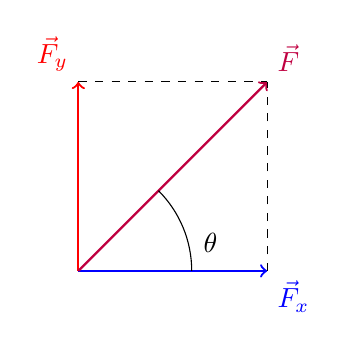
\begin{tikzpicture}[scale=1.2]
        % 原点
        \coordinate (O) at (0,0);
        % 分解的两个分力
        \draw[->, thick, blue] (O) -- (2,0) node[below right] {$\vec{F}_x$};
        \draw[->, thick, red] (O) -- (0,2) node[above left] {$\vec{F}_y$};
        % 合力
        \draw[->, thick, purple] (O) -- (2,2) node[above right] {$\vec{F}$};
        % 虚线辅助
        \draw[dashed] (2,0) -- (2,2);
        \draw[dashed] (0,2) -- (2,2);
        % 角度标记
        \draw (1.2,0) arc (0:45:1.2);
        \node at (1.4,0.3) {$\theta$};
    \end{tikzpicture}
    \end{center}

    力的合成与分解：如图所示，合力$\vec{F}$可以分解为两个垂直分力$\vec{F}_x$和$\vec{F}_y$，满足
    \[
    \vec{F} = \vec{F}_x + \vec{F}_y
    \]
    分解时常用三角函数：
    \[
    F_x = F\cos\theta,\quad F_y = F\sin\theta
    \]
}
\section{牛顿运动定律}
\concept{牛顿第二定律}{
    \[F_{\text{合}}=ma\]
    上面公式里面，$\vec{F}$表示合外力，$m$表示物体质量，$\vec{a}$表示物体加速度。这个公式很简洁，但是和前面的受力分析结合起来可以处理所有的做匀变速直线运动的物体的问题。
}
\section{动能定理}
\concept{动能定理}{
    \[W=\Delta E_k\]
    \[E_k=\frac12mv^2\]
    上面公式里面，$W$表示合外力做的功，$E_k$表示动能。
    左边是合外力做的功，右边是动能的变化量。中间过程不明确的问题可通过动能定理排除干扰，比如一个轨迹是曲线的运动，直接通过合外力的功，就能计算速度变化量，不需要中间过程的情况。
}
\section{机械能守恒定律}
\concept{机械能守恒定律}{
    \[E=E_k+E_p\]
    \[E_p=mgh+\frac12kx^2\]
    上面公式里面，$E$表示机械能，$E_k$表示动能，$E_p$表示势能，$m$表示物体质量，$g$表示重力加速度，$h$表示高度。
    机械能守恒，一般是只有弹力和重力做功的系统才生效，没有非保守力做功，比如摩擦力。
}
\section{动量定理}
\concept{动量定理}{
    \[I_{冲量}=F_{\text{合}}\Delta t\]
    \[p_{动量}=mv\]
    专门用来解决只有相互作用力的系统，如果一个系统除了相互作用力以外没有别的力，那么系统的动量守恒。否则动量不守恒，需要计算力的冲量。相比于动能定理，动量定理的适用场景更奇怪，一般是多个物体有相互作用。
}
\concept{动量守恒}{
    \[m_1v_1+m_2v_2=m_1v_1'+m_2v_2'\]
    上面公式里面，$m_1$和$m_2$表示两个物体的质量，$v_1$和$v_2$表示两个物体的初速度，$v_1'$和$v_2'$表示两个物体的末速度。
    只有相互作用力的系统动量守恒，比如碰撞问题。
    一般而言，动量守恒与机械能守恒可以同时生效，此时，可以得到机械能守恒方程：
    \[\frac12m_1v_1^2+\frac12m_2v_2^2=\frac12m_1v_1'^2+\frac12m_2v_2'^2\]
    这两个方程怎么求解呢？移项然后相除。
    比如上面的方程两边同时乘以2，然后移项得到：
    \[m_1(v_1^2-v_1'^2)=m_2(v_2'^2-v_2^2)\]
    然后两边同时除以$v_1-v_1'$和$v_2'-v_2$，得到：
    \[m_1(v_1+v_1')=m_2(v_2'+v_2)\]
    这样就得到一个新的方程，可以和动量守恒方程联立求解。
}
\end{document}